\chapter{Pushes and Pulls: Forces}\label{ch:g2:pushes-and-pulls}

Open a door, zip a zipper, kick a ball, drag a sled: your whole day
is spent pushing and pulling. Physics gathers all of these under one
proud name --- \omterm{def:g2:pushes-and-pulls:force}{force} --- and asks two simple questions: what can a
\omterm{def:g2:pushes-and-pulls:force}{force} do, and which way does it act?

\section{Pushes and pulls everywhere}

\begin{definition}[Force]\label{def:g2:pushes-and-pulls:force}
A \emph{force}\index{force} is a push or a pull. Pushing a swing,
pulling a wagon, pressing a doorbell, stretching a rubber band,
squeezing dough: every one of these is a force at work. A force
always has a strength --- gentle or mighty --- and a
\emph{direction}: it pushes or pulls \emph{some way}.
\end{definition}

\begin{example}[Push or pull?]\label{ex:g2:pushes-and-pulls:sort}
Sort your day: kicking a ball --- a push with the foot. Opening a
drawer --- a pull. Closing it --- a push. Zipping up a jacket --- a
pull. Kneading dough --- many little pushes. Tug-of-war --- two
teams pulling the same rope opposite ways.
\end{example}

\begin{method}[Drawing a force as an arrow]\label{met:g2:pushes-and-pulls:arrow}
Physicists draw a \omterm{def:g2:pushes-and-pulls:force}{force} as an \emph{arrow}:
\begin{enumerate}
  \item the arrow starts where the push or pull grabs the object;
  \item it points the way the \omterm{def:g2:pushes-and-pulls:force}{force} acts;
  \item a stronger \omterm{def:g2:pushes-and-pulls:force}{force} gets a longer arrow.
\end{enumerate}
One little arrow tells the whole story: where, which way, how hard.
We will draw these arrows for years to come.
\end{method}

\begin{omfigure}
\begin{tikzpicture}[scale=0.85]
  \draw[thick] (0,0) -- (4.6,0);
  \draw[thick, fill=omMeth, fill opacity=0.4] (1.4,0) rectangle (2.9,1.0);
  \draw[-Stealth, very thick, omThm] (0.2,0.5) -- (1.3,0.5);
  \node[below, font=\small] at (2.3,-0.25) {a gentle push: short arrow};
  \draw[thick] (6.4,0) -- (11.0,0);
  \draw[thick, fill=omMeth, fill opacity=0.4] (8.4,0) rectangle (9.9,1.0);
  \draw[-Stealth, very thick, omThm] (6.5,0.5) -- (8.3,0.5);
  \node[below, font=\small] at (8.7,-0.25) {a mighty push: long arrow};
\end{tikzpicture}

{\small The same box pushed twice. The arrow shows where the push
grabs, which way it acts, and --- by its length --- how hard.}
\end{omfigure}

\begin{omfigure}
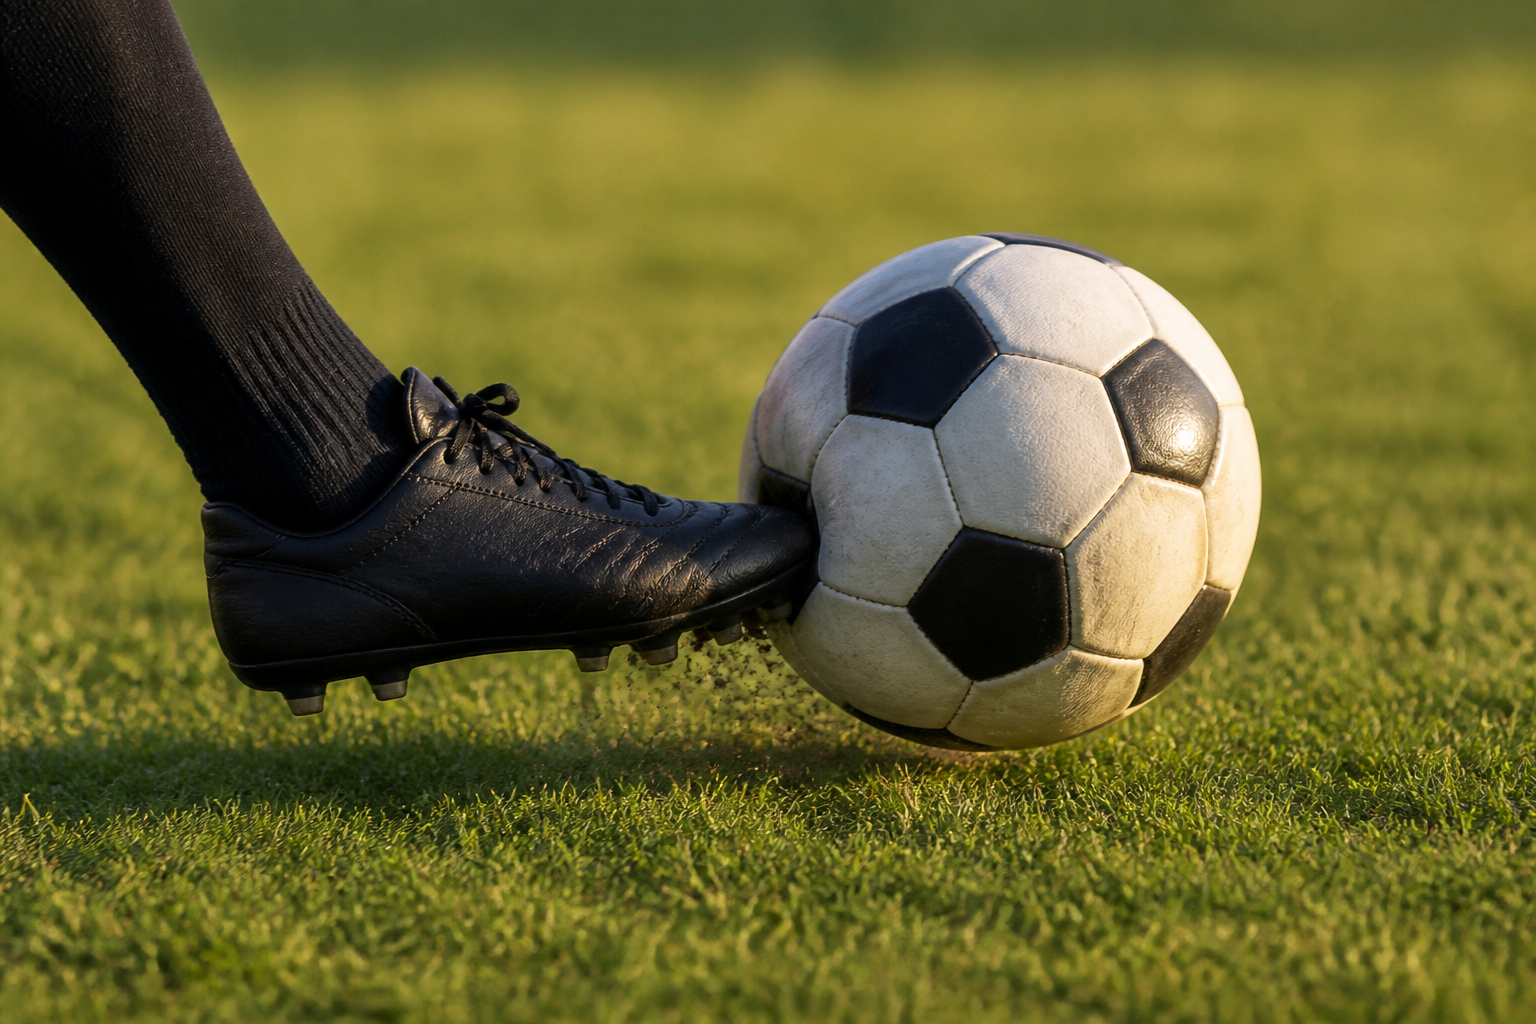
\includegraphics[width=0.58\linewidth]{images/book1/ai/g2-pushes-kick.png}

{\small A \omterm{def:g2:pushes-and-pulls:force}{force} at the moment it acts: the boot pushes, and the resting ball is about to fly.}
\end{omfigure}

\section{What forces do}

\begin{proposition}[The four jobs of a force]\label{prop:g2:pushes-and-pulls:jobs}
A \omterm{def:g2:pushes-and-pulls:force}{force} can do four things to an object:
\begin{enumerate}
  \item \emph{start} it moving --- the kick sends the resting ball
        away;
  \item \emph{stop} it --- the goalkeeper's hands stop the shot;
  \item \emph{turn} it --- a sideways tap bends the rolling ball's
        path;
  \item \emph{change its shape} --- squeezing squashes the sponge,
        pulling stretches the rubber band.
\end{enumerate}
No \omterm{def:g2:pushes-and-pulls:force}{force}, none of the four: an object left completely alone keeps
doing exactly what it was doing.
\end{proposition}

\begin{omfigure}
\begin{tikzpicture}[scale=0.85]
  \draw[dashed, omExo] (0,0.6) -- (4.2,0.6);
  \fill[omDef] (0.6,0.6) circle (0.24);
  \fill[omDef, opacity=0.45] (3.0,0.6) circle (0.24);
  \draw[-Stealth, very thick, omThm] (4.2,0.6) -- (6.0,1.7);
  \fill[omDef, opacity=0.45] (5.4,1.33) circle (0.24);
  \draw[-Stealth, thick, omThm] (4.2,-0.35) -- (4.2,0.5);
  \node[below, font=\small, omThm] at (4.2,-0.5) {sideways tap here};
  \node[below, font=\small] at (1.4,0.3) {rolling straight};
  \node[right, font=\small] at (5.85,2.05) {new direction!};
\end{tikzpicture}

{\small Job number three: a rolling ball gets a sideways tap and its
path bends toward the push.}
\end{omfigure}

\begin{example}[Stronger force, bigger effect]\label{ex:g2:pushes-and-pulls:stronger}
Tap a marble: it trundles to the table's edge. Flick it hard: it
flies across the room. Same marble, same finger --- only the
strength of the push changed, and the marble's flight changed with
it. Gentle \omterm{def:g2:pushes-and-pulls:force}{force}, gentle effect; mighty \omterm{def:g2:pushes-and-pulls:force}{force}, mighty effect.
\end{example}

\begin{example}[Try it: the shape-changers]\label{ex:g2:pushes-and-pulls:shape}
Gather a sponge, a rubber band, a lump of plasticine and a wooden
block. Squeeze and stretch each one. The sponge springs back the
moment you let go; the rubber band too. The plasticine keeps its new
shape --- your \omterm{def:g2:pushes-and-pulls:force}{force} made a dent forever. And the block? Your
strongest squeeze changes it not at all (that you can see!). Things
answer \omterm{def:g2:pushes-and-pulls:force}{force} each in their own way.
\end{example}

\section{Forces without touching}

\begin{example}[The Earth's pull]\label{ex:g2:pushes-and-pulls:earthpull}
Drop a spoon: down it goes. Toss a ball as high as you like: it
comes back down. Leaves, raindrops, crumbs --- everything let go
falls \emph{downward}. Something is pulling every one of them, all
the time, without touching them: the Earth itself. The Earth's pull
is the steadiest \omterm{def:g2:pushes-and-pulls:force}{force} in your life --- it never lets go, and it is
why ``down'' means the same thing everywhere on the playground.
\end{example}

\begin{omfigure}
\begin{tikzpicture}[scale=0.85]
  % the falling apple
  \draw[thick] (0,0) -- (5.0,0);
  \draw[thick, red!60!black, fill=red!70] (1.4,2.5) circle (0.32);
  \draw[thick, brown!60!black]
    (1.4,2.82) .. controls (1.45,2.98) .. (1.56,3.08);
  \draw[thick, green!45!black, fill=green!45]
    (1.62,3.02) ellipse [x radius=0.16, y radius=0.07, rotate=30];
  \draw[-Stealth, very thick, omDef] (1.4,2.05) -- (1.4,1.1);
  \node[right, font=\small, omDef] at (1.65,1.6)
    {the Earth pulls down};
  \node[below, font=\small] at (2.5,-0.25)
    {the apple falls: pulled, not pushed};
  % the magnet holding a paperclip up across a gap
  \draw[thick, fill=red!70] (7.9,2.35) rectangle (8.75,2.95);
  \draw[thick, fill=blue!60] (8.75,2.35) rectangle (9.6,2.95);
  \begin{scope}[shift={(8.54,1.65)}, rotate=-90]
    \draw[thick, rounded corners=2.6pt]
      (0,0) -- (1.1,0) -- (1.1,0.42) -- (0.12,0.42) -- (0.12,0.14)
      -- (0.95,0.14) -- (0.95,0.30) -- (0.30,0.30);
  \end{scope}
  \draw[-Stealth, very thick, omDef] (9.15,1.0) -- (9.15,2.0);
  \node[below, font=\small] at (8.75,0.1)
    {the magnet pulls up --- no touching};
\end{tikzpicture}

{\small Two no-touch \omterm{def:g2:pushes-and-pulls:force}{forces}: the Earth pulls the apple down through
the \omterm{def:g2:air-around-us:air}{air}; the \omterm{def:g1:magnets:magnet}{magnet} pulls the clip up through the \omterm{def:g2:air-around-us:air}{air}.}
\end{omfigure}

\begin{remark}[Old friends]\label{rem:g2:pushes-and-pulls:magnets}
You already know another no-touch \omterm{def:g2:pushes-and-pulls:force}{force}: the \omterm{def:g1:magnets:magnet}{magnet}, pulling its
paperclip across a gap of \omterm{def:g2:air-around-us:air}{air}. \omterm{def:g1:magnets:magnet}{Magnets} and the Earth's pull are the
two no-touch \omterm{def:g2:pushes-and-pulls:force}{forces} of your everyday life --- rare and precious
exceptions, for every other push or pull you meet needs contact.
Both will grow into great chapters later in this course.
\end{remark}

\section{Exercises}

\begin{exercise}[$\star$]\label{exo:g2:pushes-and-pulls:1}
Push or pull? Ringing a doorbell; \ opening a drawer; \ heading a
football; \ dragging a sled uphill; \ squeezing toothpaste.
\end{exercise}

\begin{exercise}[$\star$]\label{exo:g2:pushes-and-pulls:2}
What three things does a force-arrow tell about a \omterm{def:g2:pushes-and-pulls:force}{force}?
\end{exercise}

\begin{exercise}[$\star$]\label{exo:g2:pushes-and-pulls:3}
Name the four jobs of a \omterm{def:g2:pushes-and-pulls:force}{force}, and give your own example of each ---
different from the ones in the chapter.
\end{exercise}

\begin{exercise}[$\star$]\label{exo:g2:pushes-and-pulls:4}
A marble rolls straight toward you. Using only one finger, how do
you make it: stop? \ speed up? \ swerve to the side? Say which way
your finger pushes each time.
\end{exercise}

\begin{exercise}[$\star$]\label{exo:g2:pushes-and-pulls:5}
Which springs back and which keeps the dent: a sponge; \
plasticine; \ a rubber band; \ soft snow?
\end{exercise}

\begin{exercise}[$\star$]\label{exo:g2:pushes-and-pulls:6}
Draw a box being pushed gently to the right and the same box pushed
hard to the left. How do your two arrows differ?
\end{exercise}

\begin{exercise}[$\star$]\label{exo:g2:pushes-and-pulls:7}
What \omterm{def:g2:pushes-and-pulls:force}{force} makes every dropped thing fall? Does it need to touch the
falling spoon? Which way does it always pull?
\end{exercise}

\begin{exercise}[$\star$]\label{exo:g2:pushes-and-pulls:8}
Give the two no-touch \omterm{def:g2:pushes-and-pulls:force}{forces} you have met, each with one example
seen at home.
\end{exercise}

\begin{exercise}[$\star\star$]\label{exo:g2:pushes-and-pulls:9}
In tug-of-war, both teams pull with all their might, yet the ribbon
on the rope sometimes does not move at all. Draw the rope with the
two teams' arrows. What must be true about the two pulls when the
ribbon stands still? What happens the moment one team pulls
harder?
\end{exercise}

\begin{exercise}[$\star\star$]\label{exo:g2:pushes-and-pulls:10}
A ball thrown straight up slows, stops for an eye-blink, and falls
back. Which \omterm{def:g2:pushes-and-pulls:force}{force} is at work on the way up, at the top, and on the
way down? Does it ever stop pulling? (Draw the arrow at each of the
three moments.)
\end{exercise}
